\subsection{策略模式(Strategy)}

\subsubsection{策略模式简介}

策略模式是一种设计模式,它定义了一系列的算法,并将每一个算法封装起来,使它们可以相互替换。这样的设计模式使得算法可以在不影响到客户端的情况下发生变化。

策略模式通常被用在以下几种情况:
\begin{enumerate}
    \item 一个系统需要在多种算法中选择一种来执行。例如,一个图形处理系统可能需要不同的算法来处理不同类型的图形。
    \item 一个系统需要在多种算法中动态地选择一种来执行。例如,一个排序系统可能需要根据数据的类型和大小来选择不同的排序算法。
    \item 一个系统的算法需要随着时间的推移而发生变化。例如,一个汇率转换系统可能需要根据市场情况来选择不同的汇率计算算法。
\end{enumerate}

总之,策略模式提供了一种方便的方法来封装算法,并使得它们可以相互替换。这样,算法可以在不影响到客户端的情况下发生变化,从而提高了系统的灵活性和可扩展性。

优点:
\begin{enumerate}
    \item 策略模式提供了一种简单易懂的方法来封装算法。通过定义不同的策略类,可以轻松地在不同的算法之间进行切换。
    \item 策略模式提供了可替换算法的功能,使得客户端不需要关心具体的算法是如何实现的。这样,客户端就可以使用不同的算法来解决同一个问题,从而提高了系统的灵活性和可扩展性。
    \item 策略模式可以避免使用多重条件语句,这样可以提高代码的可读性和可维护性。
\end{enumerate}

缺点:
\begin{enumerate}
    \item 策略模式会增加系统的复杂度,因为它增加了新的策略类和上下文类。
    \item 策略模式要求客户端必须知道所有的策略类,并自行决定使用哪一个策略类。这样会增加客户端的复杂度,并且难以维护。
    \item 如果一个系统中存在大量的策略类,那么这些类可能会彼此之间重复,这样会降低代码的可重用性。
\end{enumerate}

\subsubsection{策略模式在项目中的应用}

\begin{figure}[H]
    \centering
    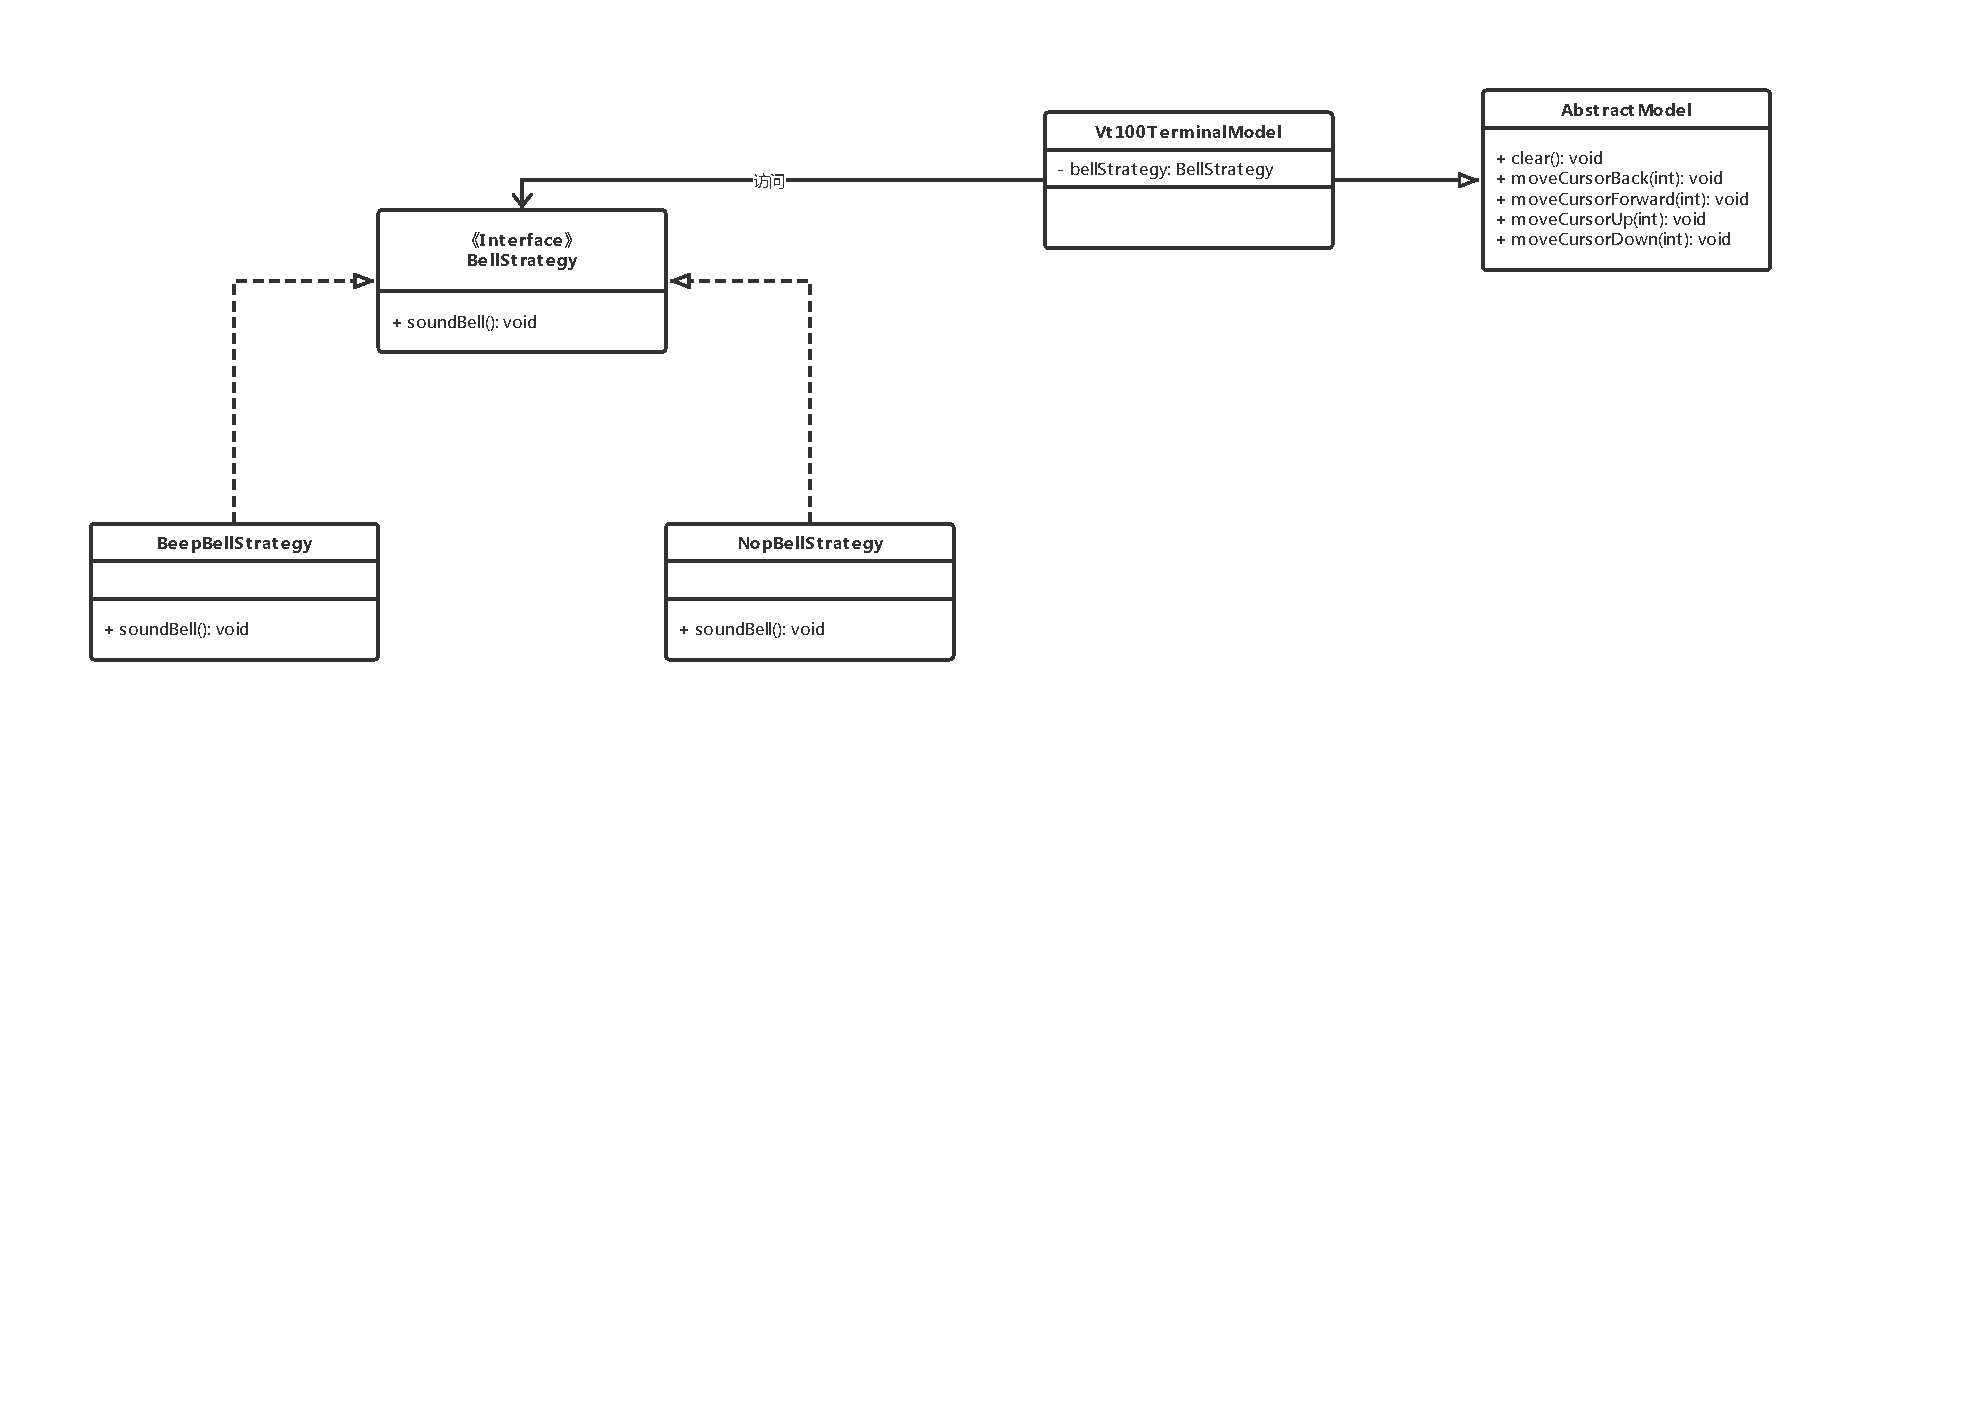
\includegraphics[width=0.9\textwidth]{figures/策略模式.pdf}
    \caption{策略模式在 Slow6502 中的类图}
\end{figure}

我们的项目中,使用策略模式实现 VT100 终端不同的蜂鸣器的行为。我们将不同的蜂鸣器行为封装起来,使它们可以相互替换,从而使得不同的蜂鸣器行为可以在不影响到调用相关功能的部分的情况下发生变化。
